\documentclass{article}
\usepackage[utf8]{inputenc}

\usepackage{csvsimple}
\usepackage{pgfplotstable,booktabs,filecontents}
\pgfplotsset{compat=1.9}% supress warning

\title{Physically-based Simulation \\ Exercise 2}
\author{ 
    Alexander Lelidis (14-907-562), \\
    Andreas Emch (08-631-384), \\
    Uro\v{s} Te\v{s}i\'{c} (17-950-346)
}
\date{\today}

\usepackage{natbib}
\usepackage{graphicx}
\graphicspath{ {images/} }

\begin{document}

\maketitle

\section{Convergence of the solution}
To find the accuracy of our implementation with compute the error between the numerical solution and the analytic solution.

\begin{equation}
v_{err} =|sol_n - sol_a|
\end{equation}

Afterwards we use the compute vector and the stiffness matrix K to get the natural norm.

\begin{equation}
|err| =\sqrt{v_{err}^t \cdot K \cdot v_{err}}
\end{equation}

This error we compute for different grid resolutions (N=3,5,8,16,32) using a graded mesh, or a regular mesh.

\newpage


\subsection{Laplace problem}
In this section we showing the errors for the Laplace problem.
\begin{equation}
- \Delta u(x,y) = 0
\end{equation}

\begin{figure}[!h]
\caption{Plot of the Poisson error}
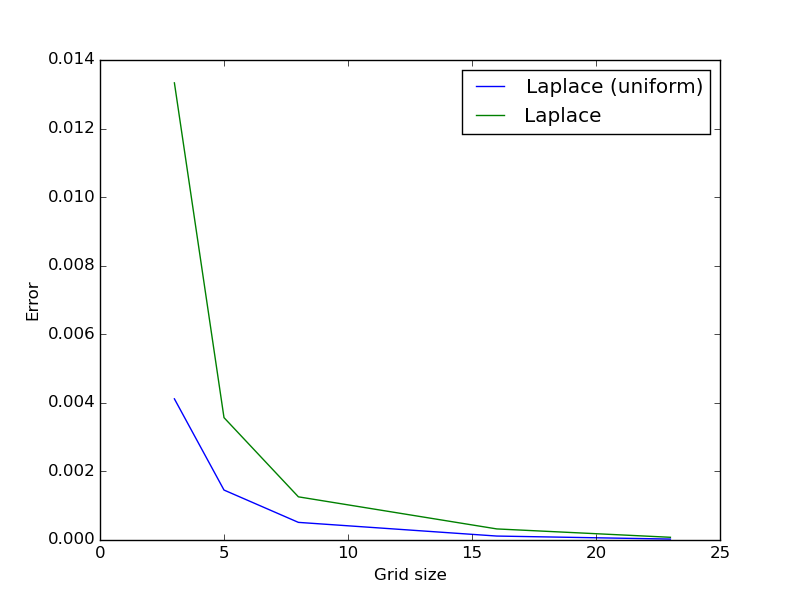
\includegraphics[width=8cm]{laplace}
\centering
\end{figure}

\newpage


\subsection{Poisson problem}
In this section we showing the errors for the Poisson problem.
\begin{equation}
- \Delta u(x,y) = f(x,y)
\end{equation}

\begin{figure}[!h]
\caption{Plot of the Poisson error}
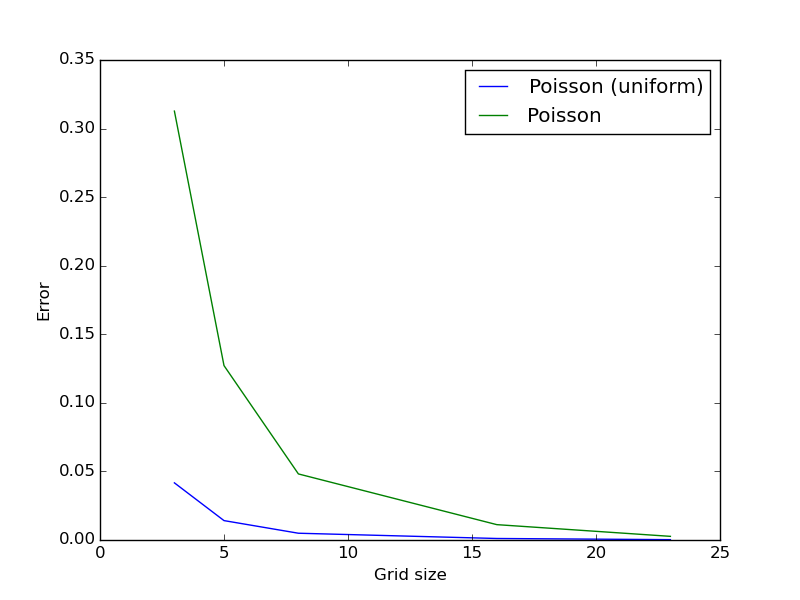
\includegraphics[width=8cm]{poisson}
\centering
\end{figure}

\end{document}
